\documentclass[oneside,numbers,spanish]{ezthesis}
%% # Opciones disponibles para el documento #
%%
%% Las opciones con un (*) son las opciones predeterminadas.
%%
%% Modo de compilar:
%%   draft            - borrador con marcas de fecha y sin im'agenes
%%   draftmarks       - borrador con marcas de fecha y con im'agenes
%%   final (*)        - version final de la tesis
%%
%% Tama'no de papel:
%%   letterpaper (*)  - tama'no carta (Am'erica)
%%   a4paper          - tama'no A4    (Europa)
%%
%% Formato de impresi'on:
%%   oneside          - hojas impresas por un solo lado
%%   twoside (*)      - hijas impresas por ambos lados
%%
%% Tama'no de letra:
%%   10pt, 11pt, o 12pt (*)
%%
%% Espaciado entre renglones:
%%   singlespace      - espacio sencillo
%%   onehalfspace (*) - espacio de 1.5
%%   doublespace      - a doble espacio
%%
%% Formato de las referencias bibliogr'aficas:
%%   numbers          - numeradas, p.e. [1]
%%   authoryear (*)   - por autor y a'no, p.e. (Newton, 1997)
%%
%% Opciones adicionales:
%%   spanish         - tesis escrita en espa'nol
%%
%% Desactivar opciones especiales:
%%   nobibtoc   - no incluir la bibiolgraf'ia en el 'Indice general
%%   nofancyhdr - no incluir "fancyhdr" para producir los encabezados
%%   nocolors   - no incluir "xcolor" para producir ligas con colores
%%   nographicx - no incluir "graphicx" para insertar gr'aficos
%%   nonatbib   - no incluir "natbib" para administrar la bibliograf'ia

%% Paquetes adicionales requeridos se pueden agregar tambi'en aqu'i.
%% Por ejemplo:
%\usepackage{subfig}
%\usepackage{multirow}
\usepackage{pdflscape}
\usepackage{booktabs}
\usepackage[utf8]{inputenc}
\usepackage{float}
%\usepackage[a4paper,margin=1in,landscape]{geometry}

%% # Datos del documento #
%% Nota que los acentos se deben escribir: \'a, \'e, \'i, etc.
%% La letra n con tilde es: \~n.

\author{
110300083 Canul Canul Cindy Guadalupe \\ 110300083@ucaribe.edu.mx \\
110300097 Kumul Uc Cristian Ariel \\ 110300097@ucaribe.edu.mx \\
110300079 Peraza Feliciano Jonathan \\ 110300079@ucaribe.edu.mx \\
}
\title{Esquemas de distribuci\'on de trabajos para un sistema ERP en la nube \\ }
\degree{}
\supervisor{\textbf{Asesor: Joel Antonio Trejo S\'anchez }}
\institution{Universidad de Alg\'un Sitio}
\faculty{Escuela de Ingenier\'ia y Ciencias}
\department{\textbf{Ingenier\'ia en Telem\'atica}}

%% # M'argenes del documento #
%% 
%% Quitar el comentario en la siguiente linea para austar los m'argenes del
%% documento. Leer la documentaci'on de "geometry" para m'as informaci'on.

%\geometry{top=40mm,bottom=33mm,inner=40mm,outer=25mm}

%% El siguiente comando agrega ligas activas en el documento para las
%% referencias cruzadas y citas bibliogr'aficas. Tiene que ser *la 'ultima*
%% instrucci'on antes de \begin{document}.
\hyperlinking
\begin{document}

%% En esta secci'on se describe la estructura del documento de la tesis.
%% Consulta los reglamentos de tu universidad para determinar el orden
%% y la cantidad de secciones que debes de incluir.

%% # Portada de la tesis #
%% Mirar el archivo "titlepage.tex" para los detalles.
%% ## Construye tu propia portada ##
%% 
%% Una portada se conforma por una secuencia de "Blocks" que incluyen
%% piezas individuales de informaci'on. Un "Block" puede incluir, por
%% ejemplo, el t'itulo del documento, una im'agen (logotipo de la universidad),
%% el nombre del autor, nombre del supervisor, u cualquier otra pieza de
%% informaci'on.
%%
%% Cada "Block" aparece centrado horizontalmente en la p'agina y,
%% verticalmente, todos los "Blocks" se distruyen de manera uniforme 
%% a lo largo de p'agina.
%%
%% Nota tambi'en que, dentro de un mismo "Block" se pueden cortar
%% lineas usando el comando \\
%%
%% El tama'no del texto dentro de un "Block" se puede modificar usando uno de
%% los comandos:
%%   \small      \LARGE
%%   \large      \huge
%%   \Large      \Huge
%%
%% Y el tipo de letra se puede modificar usando:
%%   \bfseries - negritas
%%   \itshape  - it'alicas
%%   \scshape  - small caps
%%   \slshape  - slanted
%%   \sffamily - sans serif
%%
%% Para producir plantillas generales, la informaci'on que ha sido inclu'ida
%% en el archivo principal "tesis.tex" se puede accesar aqu'i usando:
%%   \insertauthor
%%   \inserttitle
%%   \insertsupervisor
%%   \insertinstitution
%%   \insertdegree
%%   \insertfaculty
%%   \insertdepartment
%%   \insertsubmitdate

\begin{titlepage}
  \TitleBlock{
\includegraphics[height=4cm]{escudo_uni}}

  \TitleBlock{\Huge\scshape\inserttitle}
  \TitleBlock{\scshape
     \insertauthor 
     \insertdegree}
 \TitleBlock \insertsupervisor
  \TitleBlock{\textbf{Oto\~no} \textbf{\insertsubmitdate}}
  \TitleBlock[\bigskip]{\insertdepartment}
\end{titlepage}

%% Nota 1:
%% Se puede agregar un escudo o logotipo en un "Block" como:
%%   \TitleBlock{
\includegraphics[height=4cm]{escudo_uni}}
%% y teniendo un archivo "escudo_uni.pdf", "escudo_uni.png" o "escudo_uni.jpg"
%% en alg'un lugar donde LaTeX lo pueda encontrar.

%% Nota 2:
%% Normalmente, el espacio entre "Blocks" se extiende de modo que el
%% contenido se reparte uniformemente sobre toda la p'agina. Este
%% comportamiento se puede modificar para mantener fijo, por ejemplo, el
%% espacio entre un par de "Blocks". Escribiendo:
%%   \TitleBlock{Bloque 1}
%%   \TitleBlock[\bigskip]{Bloque2}
%% se deja un espacio "grande" y de tama~no fijo entre el bloque 1 y 2.
%% Adem'as de \bigskip est'an tambi'en \smallskip y \medskip. Si necesitas
%% aun m'as control puedes usar tambi'en, por ejemplo, \vspace*{2cm}.




%% # Prefacios #
%% Por cada prefacio (p.e. agradecimientos, resumen, etc.) crear
%% un nuevo archivo e incluirlo aqu'i.
%% Para m'as detalles y un ejemplo mirar el archivo "gracias.tex".
%%%% Las secciones del "prefacio" inician con el comando \prefacesection{T'itulo}
%% Este tipo de secciones *no* van numeradas, pero s'i aparecen en el 'indice.
%%
%% Si quieres agregar una secci'on que no vaya n'umerada y que *tampoco*
%% aparesca en el 'indice, usa entonces el comando \chapter*{T'itulo}
%%
%% Recuerda que aqu'i ya puedes escribir acentos como: 'a, 'e, 'i, etc.
%% La letra n con tilde es: 'n.

\prefacesection{Agradecimientos}

Este trabajo no habr'ia sido posible sin el apoyo y el est'imulo de mi colega
y amigo, Doctor Rudolf Fliesning,  bajo cuya supervisi'on escog'i este tema y
comenc'e la tesis. Sr. Quentin Travers, mi consejero en las etapas finales
del trabajo, tambi'en ha sido generosamente servicial, y me ha ayudado de
numerosos modos, incluyendo el resumen del contenido de los documentos que
no estaban disponibles para mi examen, y en particular por permitirme leer, 
en cuanto estuvieron  disponibles, las copias de los  recientes extractos de
los diarios de campa'na del Vigilante Rupert Giles y la actual Cazadora la
se'norita Buffy Summers, que se encontraron con William the Bloody en 1998, y
por facilitarme el pleno acceso  a los diarios de anteriores Vigilantes
relevantes a la carrera de William the Bloody.

Tambi'en me gustar'ia agradecerle al Consejo la concesi'on de Wyndham-Pryce
como Compa'nero, el cual me ha apoyado durante mis dos a'nos de investigaci'on,
y la concesi'on de dos subvenciones de viajes, una para estudiar documentos
en los Archivos de Vigilantes sellados en Munich, y otra para la
investigaci'on en campa'na en Praga. Me gustar'ia agradecer a Sr. Travers,
otra vez, por facilitarme  la acreditaci'on  de seguridad para el trabajo en
los Archivos de Munich, y al Doctor Fliesning por su apoyo colegial y ayuda
en ambos viajes de investigaci'on.

No puedo terminar sin agradecer a mi familia, en cuyo est'imulo constante y
amor he confiado a lo largo de mis a'nos en la Academia. Estoy agradecida
tambi'en a los ejemplos de mis  difuntos hermano, Desmond Chalmers, Vigilante
en Entrenamiento, y padre, Albert Chalmers, Vigilante. Su coraje resuelto
y convicci'on siempre me inspirar'an, y espero seguir, a mi propio y peque'no
modo, la noble misi'on por la que dieron sus vidas. Es a ellos a quien dedico
este trabajo.

%% Por si alguien tiene curiosidad, este "simp'atico" agradecimiento est'a
%% tomado de la "Tesis de Lydia Chalmers" basada en el universo del programa
%% de televisi'on Buffy, la Cazadora de Vampiros.
%% http://www.buffy-cazavampiros.com/Spiketesis/tesis.inicio.htm


%% # 'Indices y listas de contenido #
%% Quitar los comentarios en las lineas siguientes para obtener listas de
%% figuras y cuadros/tablas.

%% Los cap'itulos inician con \chapter{T'itulo}, estos aparecen numerados y
%% se incluyen en el 'indice general.
%%
%% Recuerda que aqu'i ya puedes escribir acentos como: 'a, 'e, 'i, etc.
%% La letra n con tilde es: 'n.

%\chapter*{Carta aceptaci'on}
%\addcontentsline{toc}{chapter}{Carta aceptaci'on}
%%

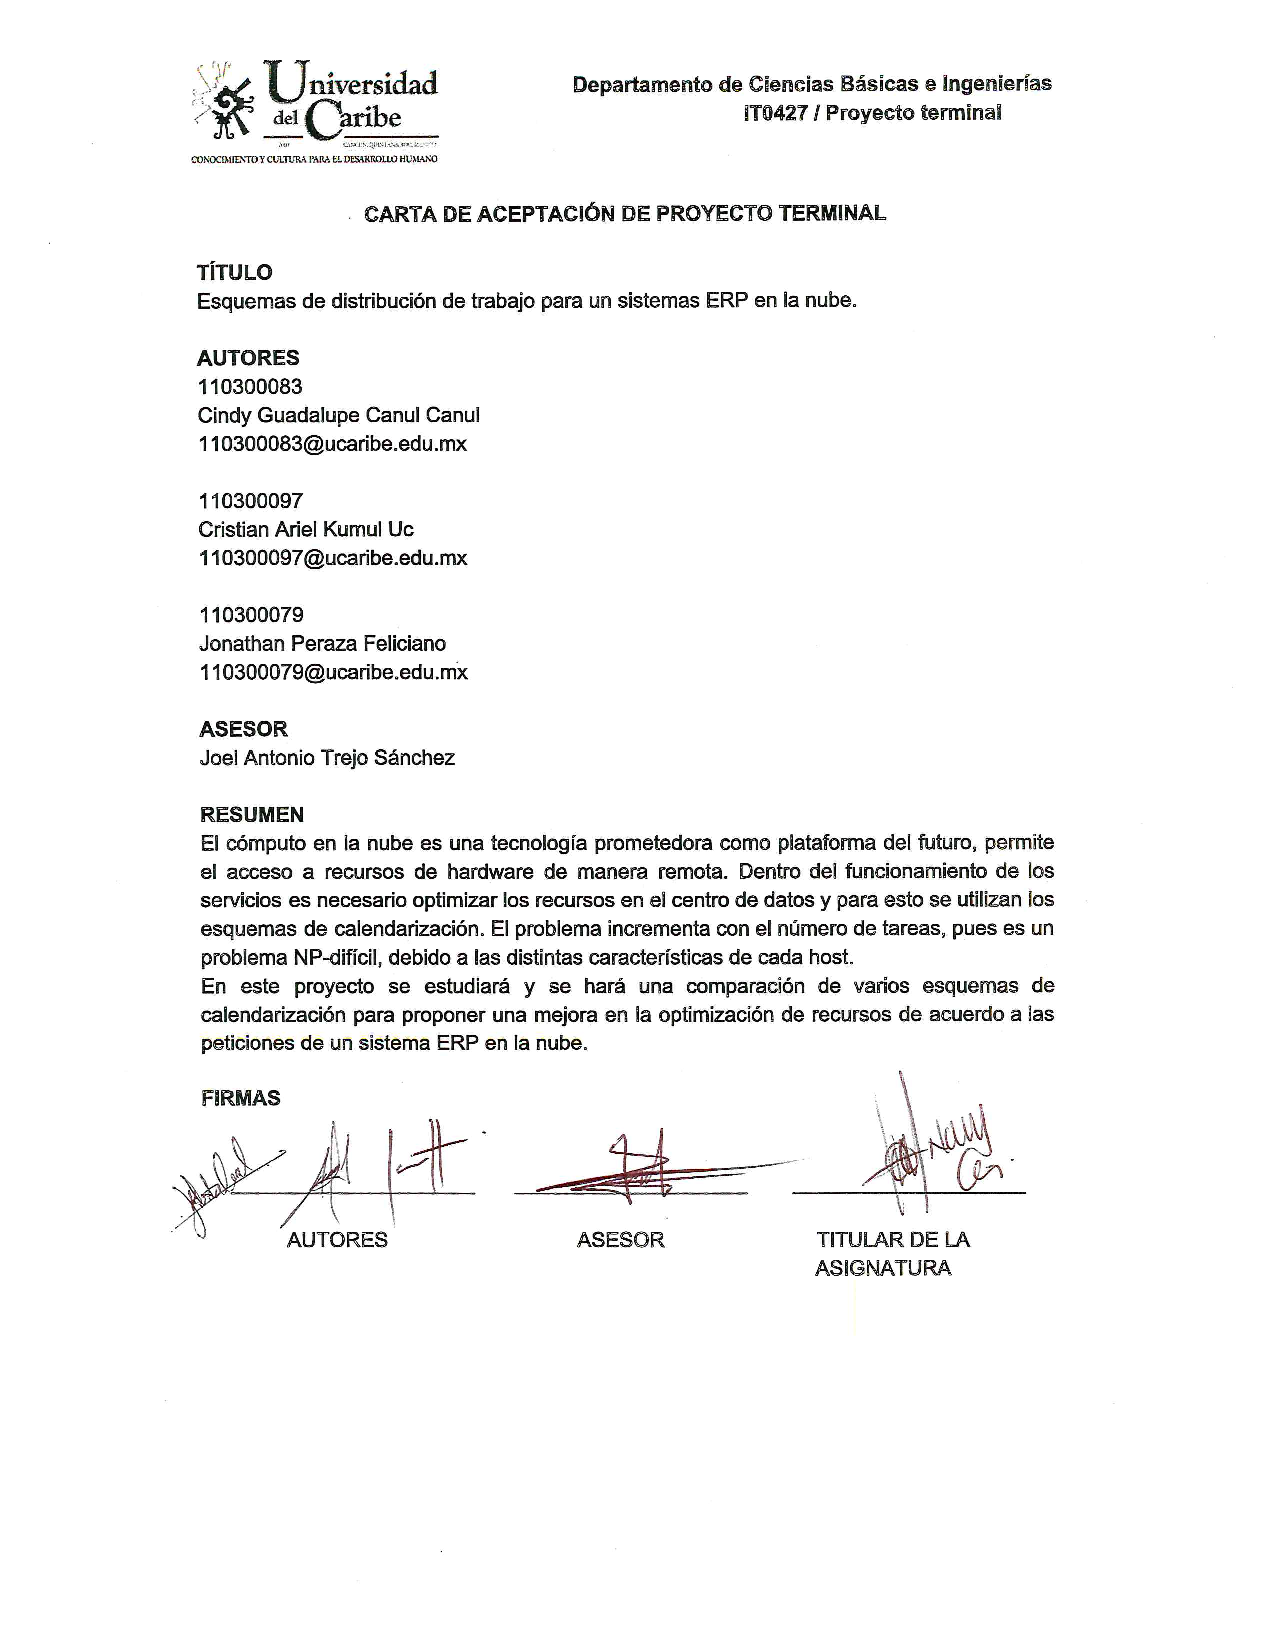
\includegraphics[width=15cm,height=20.6cm]{media/cartaceptacion.pdf}


%% Los cap'itulos inician con \chapter{T'itulo}, estos aparecen numerados y
%% se incluyen en el 'indice general.
%%
%% Recuerda que aqu'i ya puedes escribir acentos como: 'a, 'e, 'i, etc.
%% La letra n con tilde es: 'n.
\chapter*{Resumen}
\addcontentsline{toc}{chapter}{Resumen}
%%
%%\section*{Marco te'orico}
%%\addcontentsline{toc}{section}{Marco te'orico}
%%\subsection*{Cloud computing}
%%\addcontentsline{toc}{subsection}{Cloud computing}


%% Los cap'itulos inician con \chapter{T'itulo}, estos aparecen numerados y
%% se incluyen en el 'indice general.
%%
%% Recuerda que aqu'i ya puedes escribir acentos como: 'a, 'e, 'i, etc.
%% La letra n con tilde es: 'n.
\chapter*{Abstract}
\addcontentsline{toc}{chapter}{Abstract}
%%
%%\section*{Marco te'orico}
%%\addcontentsline{toc}{section}{Marco te'orico}
%%\subsection*{Cloud computing}
%%\addcontentsline{toc}{subsection}{Cloud computing}


\tableofcontents

\listoffigures
\listoftables

%% # Cap'itulos #
%% Por cada cap'itulo hay que crear un nuevo archivo e incluirlo aqu'i.
%% Mirar el archivo "intro.tex" para un ejemplo y recomendaciones para
%% escribir.

%% Los cap'itulos inician con \chapter{T'itulo}, estos aparecen numerados y
%% se incluyen en el 'indice general.
%%
%% Recuerda que aqu'i ya puedes escribir acentos como: 'a, 'e, 'i, etc.
%% La letra n con tilde es: 'n.




\chapter*{Introducci'on}
\addcontentsline{toc}{chapter}{Introducci'on}
\chaptermark{Introducci'on}

\section*{Antecedentes y Planteamiento del problema}
\addcontentsline{toc}{section}{Antecedentes y Planteamiento del problema}


El c'omputo en la nube es una tecnolog'ia que ha abarcado gran parte de los negocios  para dar soporte a ellos. 'Esta tecnolog'ia provee a los negocios una ventaja competitiva en los costos de recursos como se ve en los negocios tradicionales, adem'as de la versatilidad que provee al ajustarse a la necesidad de las empresas (\citeauthor{srinivasan2014cloud}, \citeyear{srinivasan2014cloud}).



%\cite{srinivasan2014cloud}. 

La tecnolog'ia en la nube ha desarrollado una infraestructura fuerte despu'es del surgimiento del c'omputo distribuido (\citeauthor{chen2009cloud}, \citeyear{chen2009cloud}). Para obtener las ventajas de dicha tecnolog'ia los usuarios simplemente necesitar'an conectarse a internet y de esta manera tendr'an el acceso al procesamiento de manera remota (\citeauthor{aranganathan2011aco}, \citeyear{aranganathan2011aco}). Sin embargo, para aprovechar el m'aximo potencial de 'estos recursos, es necesario tener en consideraci'on algunas variables, ya que en un entorno en la nube existe un comportamiento din'amico de los recursos a manera que se les provea a los usuarios el servicio (\citeauthor{shimpy2014different}, \citeyear{shimpy2014different}).
Una de las pr'acticas con mayor importancia en la nube es la calendarizaci'on, ya que tiene como objetivo administrar las tareas del centro de datos para optimizar los recursos del mismo. De esta manera la eficiencia de la carga de trabajo en la nube aumenta (\citeauthor{shimpy2014different}, \citeyear{shimpy2014different}).
En general, el objetivo de la calendarizaci'on en la nube es utilizar los recursos de manera apropiada, mientras la carga de trabajo es distribuida uniformemente para mejorar los tiempos de ejecuci'on (\citeauthor{shimpy2014different}, \citeyear{shimpy2014different}).
Debido a la atenci'on que se tiene en la tecnolog'ia en la nube, los centros de datos han tomado un papel muy importante para los servicios empresariales (\citeauthor{shimpy2014different}, \citeyear{shimpy2014different}). 
Un centro de datos est'a compuesto por miles de servidores virtuales ejecut'andose en una instancia de tiempo alojando muchas tareas, al mismo tiempo el centro de datos recibe miles de peticiones a esas tareas. Es aqu'i en donde la programaci'on de trabajos tiene un rol demasiado importante para el c'omputo en la nube, ya que influye en el rendimiento del mismo (\citeauthor{srinivasan2014cloud}, \citeyear{srinivasan2014cloud}). 

El problema de la calendarizaci'on pertenece a los algoritmos NP-Dif'icil, lo cual tiene un amplio rango de soluciones posibles y se toma mucho m'as tiempo de encontrar una respuesta 'optima, ya que no existe un m'etodo para resolver estas inc'ognitas. Sin embargo, es posible estar cerca de la mejor soluci'on contemplando algunos entornos (\citeauthor{shimpy2014different}, \citeyear{shimpy2014different}).




\section*{Propuesta de soluci'on y Justificaci'on}
\addcontentsline{toc}{section}{Propuesta de soluci'on y Justificaci'on}


Los centros de datos son una parte esencial en la tecnolog'ia en la nube, est'an conformados por varios servidores virtuales que alojan varios trabajos, ejecut'andose por estancias de tiempo y a la vez recibiendo peticiones a esos trabajos (\citeauthor{shimpy2014different}, \citeyear{shimpy2014different}).
Para que el c'omputo en la nube pueda rendir correctamente, se necesita una buena programaci'on de trabajos o calendarizaci'on. Este problema tiene un gran n'umero de soluciones posibles, toma mucho tiempo en encontrar un respuesta 'optima y por eso est'a dentro de los algoritmos NP-Dif'icil. No existe un m'etodo para resolver lo anterior, sin embargo es posible obtener una soluci'on cercana comtemplando algunos entornos (\citeauthor{shimpy2014different}, \citeyear{shimpy2014different}).
En esta investigaci'on se propone una mejora a un algoritmo de calendarizaci'on para el caso de estudio de un sistema ERP en la nube, contemplando sus posibles escenarios y peticiones heterog'eneas. De esta manera se podr'a contar con un esquema de distribuci'on de trabajos que satisfaga las necesidades de un sistema ERP, mejorando el tiempo de respuesta y aprovechando los recursos. Con beneficios a los proveedores de servicios (SaaS) de sistemas ERP.

\newpage

\begin{figure}
	
	\centering
	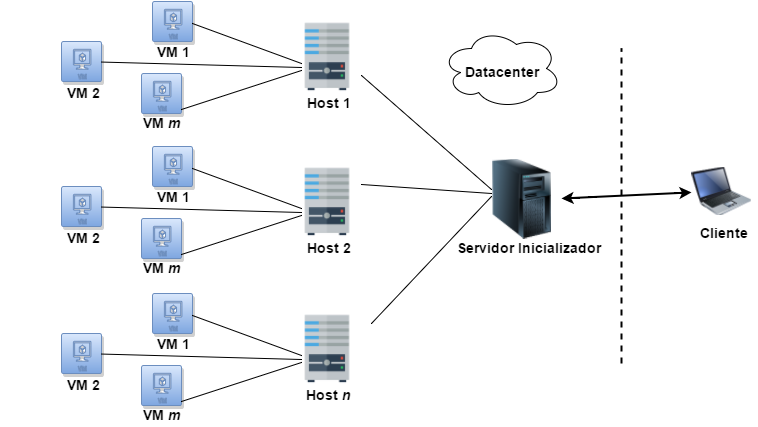
\includegraphics[scale=0.5]{media/cloud2}
	\caption{Propuesta de arquitectura en la nube, Fuente: Elaboraci'on propia. }
\end{figure}
%%%%%%%%
%%  IMAGEN
%%%


En la figura 1 se puede observar la arquitectura del centro de datos que se implementar'a en la investigaci'on, el cual est'a compuesto de los siguientes elementos:

\begin{itemize}
	\item \textbf{Servidor administrador:} Es el servidor que tendr'a el rol de front end en el centro de datos, teniendo una interacci'on directa con las peticiones de los usuarios, que son especificados en 'este documento como trabajos.
	El principal objetivo de 'este elemento es delegar los trabajos a las m'aquinas virtuales en los distintos hosts del centro de datos.
	\item \textbf{Host:} es el recurso de hardware que se tiene en el centro de datos. Una de las caracter'isticas de 'este elemento es que es finito.
	\item \textbf{M'aquinas Virtuales:} son instancias dentro de los host, tienen como objetivo resolver los trabajos que se les sea asignado.
\end{itemize}


\section*{Objetivos}
\addcontentsline{toc}{section}{Objetivos}


\subsection*{Objetivo general}
\addcontentsline{toc}{section}{Objetivo general}


Determinar y proponer un nuevo esquema que pueda resolver de manera eficiente el problema de la calendarizaci'on de un centro de datos y satisfacer las necesidades de un sistema ERP en la nube.


\subsection*{Objetivos espec'ificos}
\addcontentsline{toc}{section}{Objetivos espec'ificos}


\begin{itemize}
	\item Definir una arquitectura para un centro de datos en la nube con las necesidades de un sistema ERP.
	\item Realizar la simulaci'on en base a la arquitectura del centro de datos.
	\item Realizar e implementar diferentes esquemas de distribuci'on de trabajos, rescatando sus caracter'isticas principales.
	\item Reunir las caracter'isticas principales y proponer el nuevo esquema de distribuci'on.
	\item Aplicar el nuevo esquema de distribuci'on a las necesidades de un ERP.
	\item Comparar los resultados obtenidos del nuevo esquema propuesto y de los anteriores para determinar si hubo una mejora.
\end{itemize}


\newpage

\section*{Hip'otesis}
\addcontentsline{toc}{section}{Hip'otesis}

La modificaci'on de un esquema de distribuci'on mejorar'a el rendimiento de la calendarizaci'on para un sistema ERP en la nube.

Para realizar la verificaci'on de validez de la hip'otesis se usar'an:


\begin{itemize}
	\item \textbf{Pruebas de hardware y software:}
	\begin{itemize}
	\item \textbf{Prueba de desempe'no:} Validar el tiempo de respuesta para las tareas bajo condiciones normales y m'aximas.
	\item \textbf{Prueba de carga:} Verificar el tiempo de respuesta del sistema, bajo diferentes condiciones de carga. Se mide el tiempo de respuesta y otros requisitos sensibles al tiempo.
	\end{itemize}
	\item \textbf{Estad'isticas:} en base a los resultados que se obtendr'an en las pruebas de desempe'no y de carga, se va realizar comparaciones y posteriormente visualizarlas por medio de gr'aficas y tablas.
\end{itemize}

%% Los cap'itulos inician con \chapter{T'itulo}, estos aparecen numerados y
%% se incluyen en el 'indice general.
%%
%% Recuerda que aqu'i ya puedes escribir acentos como: 'a, 'e, 'i, etc.
%% La letra n con tilde es: 'n.

\chapter{Marco contextual}
\section*{Introducci'on}
\addcontentsline{toc}{section}{Introducci'on}

En éste cap'itulo se describen algunos marcos conceptuales necesarios para fundamentar y analizar los requisitos de la investigaci'on, las secciones son las siguientes: Situaci'on actual, Estado del Arte, Marco Te'orico y Marco Metodol'ogico. En la primera secci'on se muestra c'omo se encuentra la investigaci'on en la actualidad, c'omo se encuentra nacional e internacionalmente y cu'al es el punto de partida del proyecto; en la siguiente secci'on se presenta la informaci'on sobre los diferentes esquemas de distribuci'on que ser'an implementados durante la elaborac'on del proyecto. El Marco te'orico nos describe los conceptos necesarios para fundamentar y comprender mejor el proyecto y su prop'osito, finalmente en la 'ultima secci'on se describe los pasos que se van a seguir para realizar y alcanzar los objetivos del proyecto.

\newpage


\section{Situaci'on Actual}

Actualmente, hay un mayor n'umero de organizaciones que utilizan el c'omputo en la nube, ya que trae beneficios en cuanto a gastos y recursos. Ya no hay necesidad de invertir tanto en la administraci'on de TI (Information Technology) y existe una mejor capacidad de almacenamiento para los recursos que el 'ambito empresarial necesita.
El c'omputo en la nube utiliza los servicios SaaS (Software as a Service) y HaaS (Hardware as a Service) para hacer m'as eficiente y flexible el uso de la infraestructura de la nube (\citeauthor{mariscal2013computo}, \citeyear{mariscal2013computo}). 

M'exico utiliza, en cuanto a la infraestructura, los servicios ofrecidos por Amazon, Google y Triada (TELMEX). Estos proporcionan almacenaje de informaci'on virtual, plataformas de hospedaje de aplicaciones y servicios en l'inea (\citeauthor{mariscal2013computo}, \citeyear{mariscal2013computo}).

Al proveer el servicio se tiene dos escenarios diferentes: cuando hay una mayor demanda de recursos y cuando no la hay,  eso va dependiendo de las necesidades de las empresas. 
Para que se tenga una mejor eficacia durante los servicios, se tiene que mejorar el uso de los recursos en el centro de datos. Dentro del centro de datos hay muchos servidores virtuales que est'an recibiendo trabajos, mientras la nube las mantiene en los lotes de solicitud de trabajos. Es aqu'i, donde resaltamos la importancia de la distribuci'on de trabajos dentro del centro de datos (\citeauthor{shimpy2014different}, \citeyear{shimpy2014different}). 

En este momento, la distribuci'on de trabajos es un problema NP- dif'icil, pues que no se ha encontrado una soluci'on 'optima. Sin embargo, existen diferentes propuestas para encontrar una mejor soluci'on, utilizando diferentes esquemas de distribuci'on o dicho de otra forma algoritmos (\citeauthor{shimpy2014different}, \citeyear{shimpy2014different}). 

Existen una gran variedad de algoritmos utilizados en el problema de distribuci'on de trabajos. Los algoritmos m'as utilizados en las investigaciones son: FCFS, Round Robin, Min-Min, Max-Min y Metaheur'istica. Cabe mencionar que en las investigaciones solo hacen una selecci'on de una serie de algoritmos para que, por medio de pruebas, determinen qui'en es el mejor de ellos. 


\newpage
\section{Estado del Arte}


Los siguientes algoritmos de calendarizaci'on actualmente est'an prevaleciendo en la nube:
\begin{itemize}
	\item \textbf{Resource-Aware-Scheduling Algorithm (RASA):} Parsa, Entezari-Maleki (2009) proponen el algoritmo RASA, el cual utiliza las ventajas de dos algoritmos tradicionales (Max-min y Min-min) y cubre sus desventajas. Aunque el tiempo limite, la tasa de llegada, costo de ejecucion y costo de comunicaci'on no est'an considerados (\citeauthor{parsa2009rasa}, \citeyear{parsa2009rasa}).
	
	
	\item \textbf{RSDC (Reliable Scheduling Distributed In Cloud Computing):} Delevar, Javanmard, Shabestari y Talebi (2012) proponen un algoritmo confiable en un entorno en la nube, en este algoritmo los trabajos importantes son divididos en sub trabajos, de tal manera que se puedan balancear las peticiones (\citeauthor{delavar2012rsdc}, \citeyear{delavar2012rsdc}).
	
	
	\item \textbf{An Optimal Model for Priority based Service Scheduling Policy for Cloud Computing Environment:} Dakshayini, Gurupased (2011), proponen un nuevo algoritmo de calendarizaci'on que se basa en la prioridad y un esquema de control de admisi'on. En este algoritmo, la prioridad se asigna a cada proceso admitido en la cola (\citeauthor{dakshayini2011optimal}, \citeyear{dakshayini2011optimal}) . 
	
	
	\item \textbf{Pre-emptable Shortest Job Next Scheduling algorithm (PSJN) :}  Este algoritmo se propone en una nube privada. Utiliza la t'ecnica de suscripci'on preferente del algoritmo de Round Robin junto con el siguiente proceso m'as corto (PSN). Brinda beneficios de costos y mejora tiempo de respuesta y tiempo de ejecuci'on (\citeauthor{nishant}, \citeyear{nishant}). 
	
	
	\item \textbf{User-priority Guided Min-min scheduling algorithm:} Se realiza una mejora para el algoritmo de balanceo de cargas, a trav'es del algoritmo Min-min para la calendarizaci'on de trabajos con el fin de minimizar el tiempo de terminaci'on del ultimo trabajo (makespan) y maximizar la utilizaci'on de los recursos (\citeauthor{chen2013user}, \citeyear{chen2013user}). 
\end{itemize}



\section{Marco te'orico}

El c'omputo en la nube es una tecnolog'ia emergente, la cual est'a compuesta por un grupo de recursos heterog'eneos que proveen servicios a trav'es de internet (\citeauthor{agarwal2014efficient}, \citeyear{agarwal2014efficient}).
Esta tecnolog'ia permite a los consumidores y negocios utilizar aplicaciones sin necesidad de instalaci'on y con acceso a sus archivos personales en cualquier computadora con acceso a internet (\citeauthor{ahmed2012advanced}, \citeyear{ahmed2012advanced}). 
El c'omputo en la nube se puede clasificar de dos maneras:
\begin{itemize}
	\item Por la ubicaci'on: 
	\begin{itemize}
		\item \textbf{Nube P'ublica:} La infraestructura de c'omputo se puede compartir entre cualquier organizaci'on (\citeauthor{ahmed2012advanced}, \citeyear{ahmed2012advanced}).
		\item \textbf{Nube Privada:} La infraestructura de c'omputo es dedicada a una organizaci'on en particular y no se comparte con otras organizaciones (\citeauthor{ahmed2012advanced}, \citeyear{ahmed2012advanced}).
		\item \textbf{Nube H'ibrida:} Las organizaciones pueden albergar sus aplicaciones cr'iticas en nubes privadas y las aplicaciones con menos problemas de seguridad las puede albergar en nubes p'ublicas (\citeauthor{ahmed2012advanced}, \citeyear{ahmed2012advanced}).
	\end{itemize}
	\item Por el tipo de servicios ofrecidos: 
	\begin{itemize}
		\item \textbf{Infrastructure as a Service (IaaS):} En 'este nivel, la infraestructura se ofrece como servicio hacia los solicitantes en forma de M'aquinas Virtuales (VM) (\citeauthor{agarwal2014efficient}, \citeyear{agarwal2014efficient}).
		\item \textbf{Platform as a Service (PaaS):} Es una plataforma de desarrollo de aplicaciones que se provee como servicio hacia los desarrolladores para crear aplicaciones basadas en web (\citeauthor{agarwal2014efficient}, \citeyear{agarwal2014efficient}).
		\item \textbf{Software as a Service (SaaS):} En 'este nivel el proveedor en la nube provee las aplicaciones de software (\citeauthor{agarwal2014efficient}, \citeyear{agarwal2014efficient}).
	\end{itemize}
\end{itemize}



%%%%%
%%%%%%%%% INSERTAR IMAGEN DEL DRIVE AQUI!
\begin{figure}
	\caption{Esquema general del C'omputo en la Nube, Fuente: Elaboraci'on propia.}
	\centering
	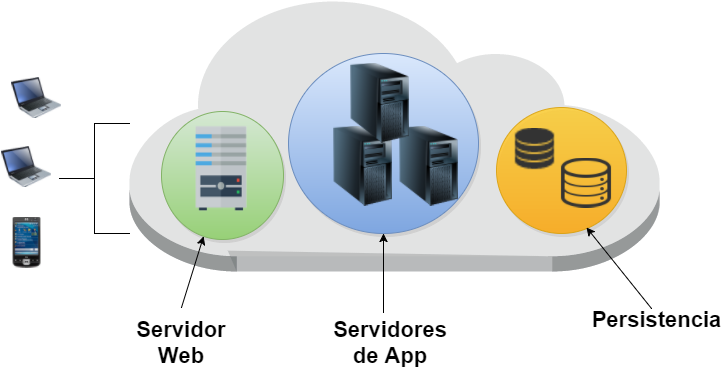
\includegraphics[scale=0.5]{media/cloud1}
\end{figure}
\subsection*{Centro de Datos}
\addcontentsline{toc}{subsection}{Centro de Datos}
Un centro de datos (datacenter) es un espacio dedicado donde las organizaciones almacenan y operan la mayor'ia de su informaci'on y la infraestructura de las tecnolog'ias de comunicaciones que respaldan sus negocios (\citeauthor{whatisdatacenter}, \citeyear{whatisdatacenter}).

\subsection*{Esquemas de Distribuci'on de Trabajos}
\addcontentsline{toc}{subsection}{Esquemas de Distribuci'on de Trabajos}

La distribuci'on de trabajo (calendarizaci'on) es uno de los puntos principales adem'as de los m'as retadores problemas en el c'omputo en la nube (\citeauthor{li2014greedy}, \citeyear{li2014greedy}). Esta consiste en un conjunto de pol'iticas para controlar el orden en el cual los procesos ser'an ejecutados por el sistema (\citeauthor{agarwal2014efficient}, \citeyear{agarwal2014efficient}).

Existen varios tipos de algoritmos de calendarizaci'on, su principal ventaja es obtener un alto rendimiento al cumplir con las trabajos. Los principales ejemplos de algoritmos de calendarizaci'on son (\citeauthor{salot2013survey}, \citeyear{salot2013survey}):

\begin{itemize}
	\item \textbf{FCFS (First Come First Serve) Algorithm:} significa que el trabajo que llegue primero ser'a el primero en ser ejecutado.
	\item \textbf{Round Robin Algorithm:} consiste en agregar un tiempo de ejecuci'on para cada trabajo, si dicho tiempo se agota y el trabajo actual no ha finalizado, pasa a un estado de espera y contin'ua con el siguiente trabajo, al finalizar el 'ultimo trabajo regresa a revisar si existen trabajos en espera para proceder a ejecutarlas. 
	\item  \textbf{Min-Min Algorithm:} se va ejecutando una por una iniciando por los trabajos de menor tama'no.
	\item  \textbf{Max-Min Algorithm:} se va ejecutando una por una iniciando por los trabajos de mayor tama'no.
	\item  \textbf{Most fit task scheduling algorithm:} este algoritmo busca los elementos m'as aptos en la cola de trabajos para ejecutarlo primero. Tiene un alto r'adio de error.
	\item \textbf{Priority scheduling algorithm:} la idea b'asica es que a cada proceso se le asigna una prioridad, y dependiendo a las prioridades de los dem'as procesos es c'omo se ejecutar'an cada uno de ellos.
\end{itemize}

\subsection*{Balanceo de Cargas}
\addcontentsline{toc}{subsection}{Balanceo de Cargas}

Dentro de nuestro entorno en la nube cada host tiene recursos de hardware finitos y son susceptibles a fallos. Para mitigar contra las fallas y el exhaustivo uso de los recursos, los host son agrupados en clusters, los cuales son esencialmente un agrupamiento de recursos compartidos. El administrador (manager) es capaz de asegurarse que ninguno de los host dentro del cluster es responsable de todas las m'aquinas virtuales dentro de ese cluster (\citeauthor{redhat}, \citeyear{redhat}).

Un entorno de virtualizaci'on responde a los cambios en la demanda para los recursos en cada host haciendo uso del balanceo de cargas, calendarizaci'on de trabajos y migraci'on.

Una pol'itica de balanceo de cargas es configurada para un cluster, que a su vez contiene multiples hosts, cada uno de ellos con distintos recursos de hardware y disponibilidad de memoria (\citeauthor{redhat}, \citeyear{redhat}). 
Existen tres pol'iticas para el balanceo de cargas:
\begin{itemize}
	\item Sin Balanceo.
	\item Distribuci'on Uniforme.
	\item Ahorro de Energ'ia.
\end{itemize}

\subsection*{Migraci'on}
\addcontentsline{toc}{subsection}{Migraci'on}

La migraci'on se utiliza para hacer cumplir las pol'iticas dentro del balanceo de cargas. La migraci'on de una m'aquina virtual toma lugar de acuerdo a las pol'iticas de balanceo de cargas para un cluster y la demanda actual sobre los hosts dentro de dicho cluster. La migraci'on de igual manera puede ser configurada para ocurrir autom'aticamente cuando un host es bloqueado o movido a modo de mantenimiento (\citeauthor{redhat}, \citeyear{redhat}).
\subsection*{Sistemas ERP}
\addcontentsline{toc}{subsection}{Sistemas ERP}

La sigla ERP, en ingl'es Enterprise Resource Planning, significa Planificaci'on de los Recursos de la Empresa. Un sistema ERP constituye un marco de trabajo que incluye aplicaciones comerciales, administrativas (finanzas, contabilidad), recursos humanos, planeamiento de manufactura y gesti'on de proyectos (\citeauthor{saroka2002sistemas}, \citeyear{saroka2002sistemas}). 


\section{Marco Metodol'ogico}

A continuaci'on se propone la siguiente metodolog'ia para llevar a cabo el proyecto:

\begin{itemize}
	\item \textbf{Simular:} Se implementar'a a manera de simulaci'on un centro de datos con un entorno en la nube, las m'aquinas virtuales y el servidor inicializador que lo conforman.
	\item \textbf{Implementar:} En el centro de datos se desarrollar'an los algoritmos de calendarizaci'on que se mencionan con antelaci'on.
	\item \textbf{Evaluar:} Se simular'a el comportamiento de las peticiones de un sistema contemplando los distintos escenarios del ERP y consumiendo el servicio en la nube (SaaS), para conocer el rendimiento en tiempo de ejecuci'on de los algoritmos.
	\item \textbf{Mejorar:} Se propondr'a una mejora a alg'un algoritmo de acuerdo a las necesidades y comportamiento de un sistema ERP en la nube.
	\item \textbf{Comparar:} Se realizar'a una comparativa de tiempo de ejecuci'on entre la versi'on mejorada y la original para el caso de estudio de un sistema ERP.
\end{itemize}





\chapter{Desarrollo}
\section*{Introducci'on}

En 'este cap'itulo se muestra la arquitectura de los distintos esquemas de calendarizaci'on de trabajos en un entorno en la nube, para la implementaci'on de dichos esquemas hace uso de un framework llamado CloudSim, el cual será definido de igual manera.


\newpage


\addcontentsline{toc}{section}{Introducci'on}
\section{Aplicaci'on del marco metodol'ogico y de actividades de experimentaci'on}

En base de los dos primeros puntos descritos anteriormente en el marco metodol'ogico se realizar'on las siguientes activides:

\begin{itemize}
	\item \textbf{Simular:} Se implementar'a a manera de simulaci'on un centro de datos con un entorno en la nube, las m'aquinas virtuales y el servidor inicializador que lo conforman.
	\item \textbf{Implementar:} En el centro de datos se desarrollar'an los algoritmos de calendarizaci'on que se mencionan con antelaci'on.
\end{itemize}

\subsection{Simulaci'on del Centro de Datos en la Nube}

 \textbf{Cloudsim} es un nuevo, generalizado y extensible framework de simulaci'on, que permite el modelaje, simulaci'on y experimentaci'on de infraestructuras emergentes de c'omputo en la nube y servicios de aplicaci'on. (Calheiros et al, 2010, p.2).

Entre los componentes que proporciona dicho framework se encuentran los siguientes (Calheiros et al, 2010, cap. 4):

\begin{itemize}
	\item  \textbf{Cloudlet:} Esta clase modela las aplicaciones de servicio basadas en la nube como pueden ser env'io de contenido, redes sociales, y flujo de trabajo empresarial.
	\item  \textbf{Datacenter:} Esta clase modela el nucleo de los servicios en un nivel de infraestructura (hardware) que son ofrecidos por Cloud Providers (Amazon, Azure, App Engine). Estos son encapsulados en un conjunto de host que pueden ser homogeneos o heterogeneos con respecto a sus configuraciones de hardware (memoria, n'ucleos, capacidad, y almacenamiento).
	\item  \textbf{DatacenterBroker:} Esta clase modela un broker, el cual es responsable de mediar las negociaciones entre el SaaS y los Cloud providers; y dichas negociaciones son manejadas por los requerimientos QoS.
	\item  \textbf{Host:} Esta clase modela los recursos físicos como una computadora o un servidor de almacenamiento.
	\item  \textbf{Vm:} Esta clase modela una M'aquina Virtual (VM), la cual es adinistrada y hosteada por un componente host en la nube. Cada VM tiene acceso a un componente que almacena las siguientes características relacionadas a una VM: memoria accesible, procesador, tama'no de almacenamiento.
\end{itemize}


\begin{figure}
	\caption{Estilo de Trabajo de Cloudsim, Fuente: Chatterjee et al.}
	\centering
	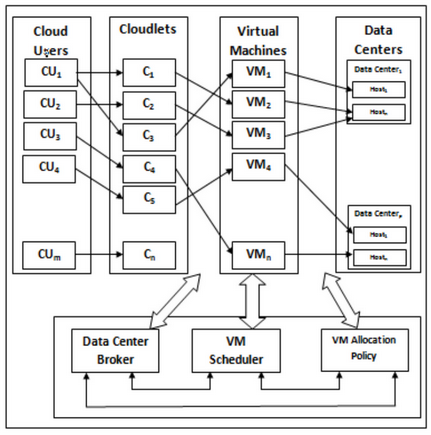
\includegraphics[scale=0.5]{media/imagenuno}
\end{figure}


\subsection{Implementaci'on de los Algoritmos}

Existen varios algoritmos para calendarizar los trabajos en el c'omputo en la nube. La mayor ventaja de estos algoritmos es obtener el mayor rendimiento. Los principales ejemplos de algoritmos de calendarizaci'on son: FCFS, Round Robin, Min-Min, Max-Min y algoritmos de meta heurísticas.(Shimpy y Jagandeep, 2014, p. 1).

De los algoritmos mencionados anteriormente en 'este trabajo se presentan los siguientes:


\begin{itemize}
	\item  \textbf{FCFS:} Ejecuta las tareas en orden de llegada, es decir, el primero en llegar es el primero en ser atendido.
	\item  \textbf{Min-Min:} Selecciona las tareas m'as pequeñas para ser ejecutadas primero.
	\item  \textbf{Max-Min:} Selecciona las tareas m'as grandes para ser ejecutadas primero.
\end{itemize}

En un entorno de trabajo normal, la forma descrita anteriormente la podemos ver de la siguiente manera:

\begin{figure}
	\caption{Esquema de trabajo de algoritmos de calendarización
		Fuente: Elaboración propia.}
	\centering
	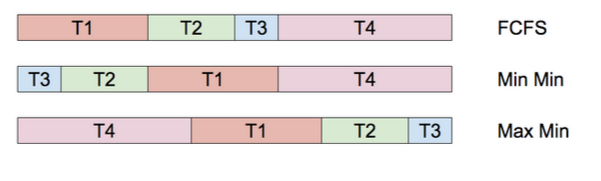
\includegraphics[scale=0.5]{media/imagendos}
\end{figure}


\newpage
Sin embargo, en un entorno en la nube al ser m'ultiples m'aquinas virtuales alojadas en distintos hosts que a su vez pueden formar parte de uno o más datacenters dicho esquema tiene que ser adaptado para poder adoptar un estilo de trabajo similar al proporcionado por nuestro framework, por lo que los resultados quedan de la distinta manera:

\begin{figure}
	\caption{Arquitectura FCFS para un entorno en la nube. Fuente: Elaboración propia.}
	\centering
	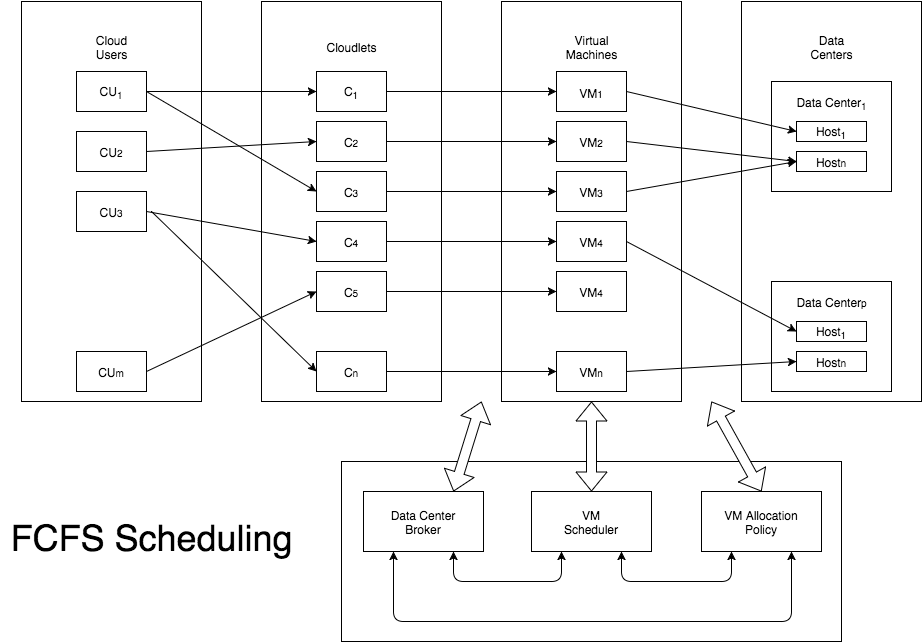
\includegraphics[scale=0.5]{media/imagentres}
\end{figure}

Como podemos apreciar en el diagrama, podemos tener m usuarios ejecutando \emph{n} tareas, sin embargo la asignaci'on de m'aquinas virtuales va dependiendo del orden de llegada de dichas tareas, y quien se encarga de repartir las tareas es el datacenterBroker.

De manera similar tenemos los siguientes algoritmos min-min y max-min:



\begin{figure}
	\caption{Arquitectura de Max-Min para un entorno en la nube. Fuente: Elaboración propia.}
	\centering
	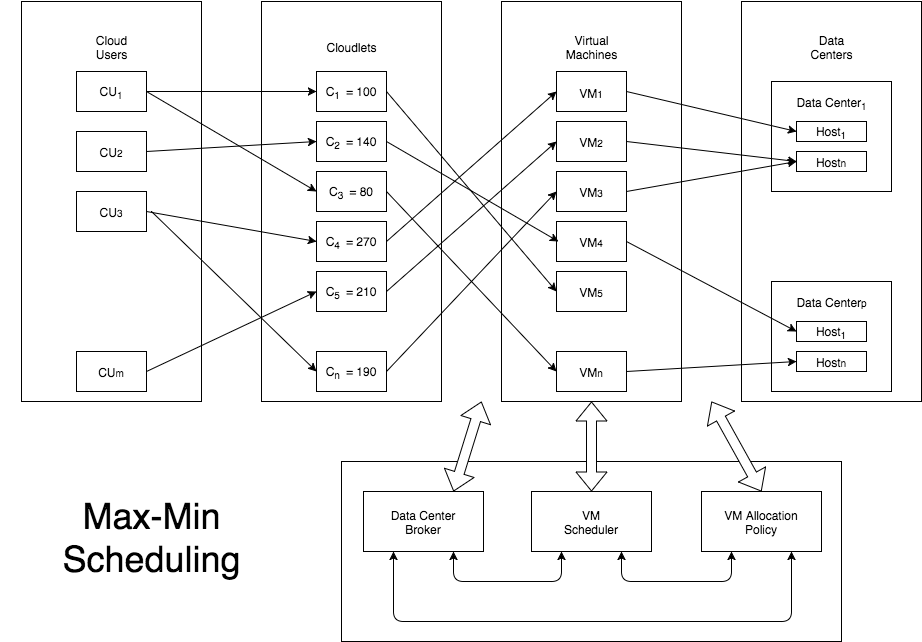
\includegraphics[scale=0.5]{media/imagencuatro}
\end{figure}


\begin{figure}
	\caption{Arquitectura de Min-Min para un entorno en la nube. Fuente: Elaboración propia.}
	\centering
	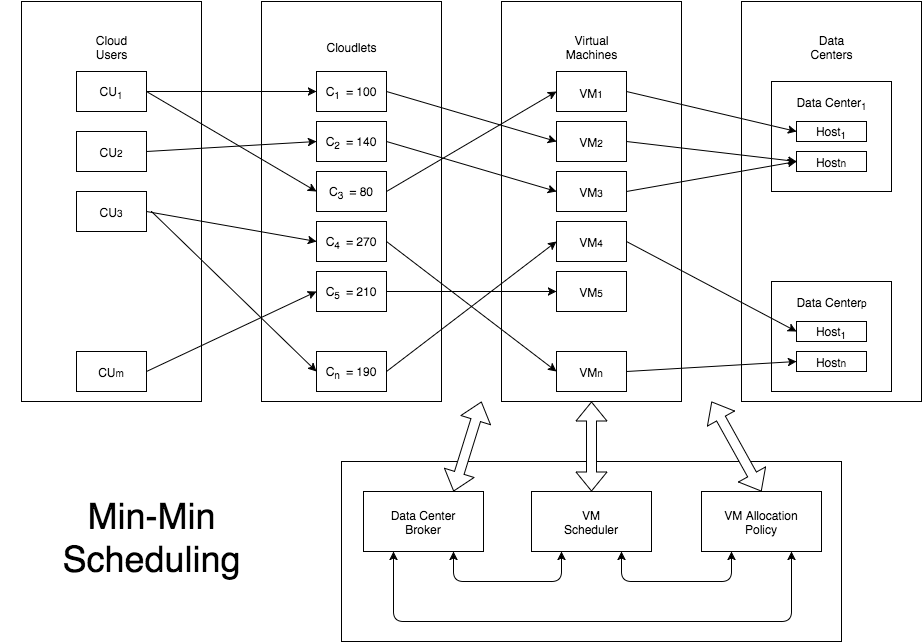
\includegraphics[scale=0.5]{media/imagencinco}
\end{figure}

\chapter{Resultados}
\section*{Introducci'on}
\addcontentsline{toc}{section}{Introducci'on}

En 'este cap'itulo se describir'an los resultados obtenidos en modelado y simulaci'on del centro de datos en CloudSim. La experimentaci'on fue desarrollada en una computadora con  un procesador Intel Core i5  con la siguiente configuraci'on: 2.5 GHz, 3 MB de cach'e, 4 GB de RAM , Linux Ubuntu 14.04 lts 64 bits como sistema operativo y JDK 8.6.
\bigskip
Para evaluar los algoritmos de calendarizaci'on seleccionados se ha implementado un entorno de c'omputo en la nube que consiste en un datacenter,un broker, m'aquinas virtuales y host.  Con el objetivo de evaluar el tiempo de ejecuci'on y el costo de procesamiento en el datacenter tras ejecutar ciertos n'umero de tareas (cloudlets).



\begin{table}[]
	\centering
	\caption{Configuraci'on Datacenter}
	\label{my-label}
	\begin{tabular}{@{}cc@{}}
		\toprule
		\multicolumn{2}{c}{{\bf Datacenter}} \\ \midrule
		Host              & 10               \\
		VM                & 5                \\
		Cloudlet          & 100-500          \\ \bottomrule
	\end{tabular}
\end{table}



Para la configuraci'on del centro de datos en CloudSim se utilizaron diez host, cinco m'aquinas virtuales por host y las tareas fueron establecidas en un intervalo de 100 – 500 (tabla 3.1).
Como se puede apreciar en la tabla 3.2, cada host tuvo 2048 Mb de memoria RAM, Dos n'ucleos de procesamiento, de almacenamiento de 800 GB o 1TB elegidas de manera aleatoria, el ancho de banda fue de 1GB/s.

\begin{table}[]
	\centering
	\caption{Configuraci'on de Host}
	\label{my-label}
	\begin{tabular}{@{}cc@{}}
		\toprule
		\multicolumn{2}{c}{{\bf Host}} \\ \midrule
		RAM           & 2048 MB        \\
		CPU           & 2              \\
		Storage       & 800GB-1TB      \\ \midrule
		BW            & 1 GB/s        
	\end{tabular}
\end{table}

En la tabla 3.3 se muestran los par'ametros que se consider'o para las m'aquinas virtuales, donde cada VM tendr'a 10 GB de almacenamiento, 512 MB  o 1 GB seleccionado de manera aleatoria, adem'as para la caracter'istica del procesador se tiene  la propiedad MIPS (million instructions per second) con 250 o 500 y un ancho de banda de 1000kb/s.


\begin{table}[]
	\centering
	\caption{My caption}
	\label{my-label}
	\begin{tabular}{@{}cc@{}}
		\toprule
		\multicolumn{2}{c}{{\bf VirtualMachine}} \\ \midrule
		RAM               & 512 MB| 1GB          \\
		MIPS              & 250 | 500            \\
		Storage           & 10 GB                \\ \midrule
		BW                & 1 GB/s              
	\end{tabular}
\end{table}
\bigskip
Para la configuraci'on de las tareas, se tom'o el tama'no con un intervalo de 1kb a 10kb,  el par'ametro fileSize que representa el tama'no del archivo de entrada va de 300b a 1.8kb as'i como el archivo de salida, como par'ametro final se tiene los MIPS que ir'an de 1 a 3.



\begin{table}[]
	\centering
	\caption{Configuraci'on Cloudlet}
	\label{my-label}
	\begin{tabular}{@{}cc@{}}
		\toprule
		\multicolumn{2}{c}{{\bf Cloudlet}} \\ \midrule
		length           & 1kb-10kb        \\
		MIPSlength       & 300b-1.8kb      \\
		length           & 300b-1.8kb      \\ \midrule
		length           & 1000 kb/s      
	\end{tabular}
\end{table}

\begin{figure}
	\caption{Promedio tiempo de ejecuci'on con tareas 100-500}
	\centering
	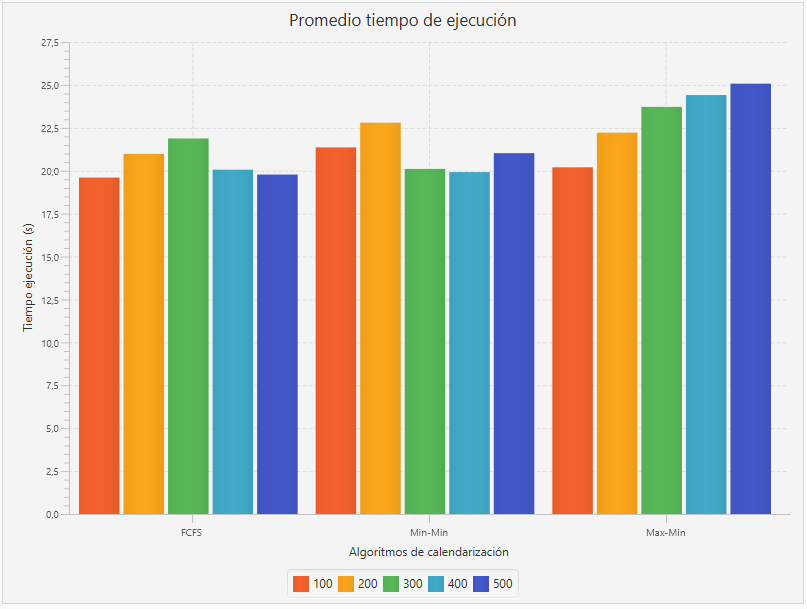
\includegraphics[scale=0.5]{media/tiempoejecucion}
\end{figure}

En la figura 3.1, se puede observar el promedio del tiempo de ejecuci'on en ms para diferentes cantidades de tareas (de 100 a 500). A primera vista con el algoritmo FCFS y Min-Min se mantiene un tiempo de ejecuci'on sin muchos cambios a pesar del aumento en la carga de tareas, a diferencia del algoritmo Max-Min que aument'o el tiempo de ejecuci'on a medida que se increment'o el n'umero de tareas.

\begin{figure}
	\caption{Promedio costo de procesamiento con tareas 100-500}
	\centering
	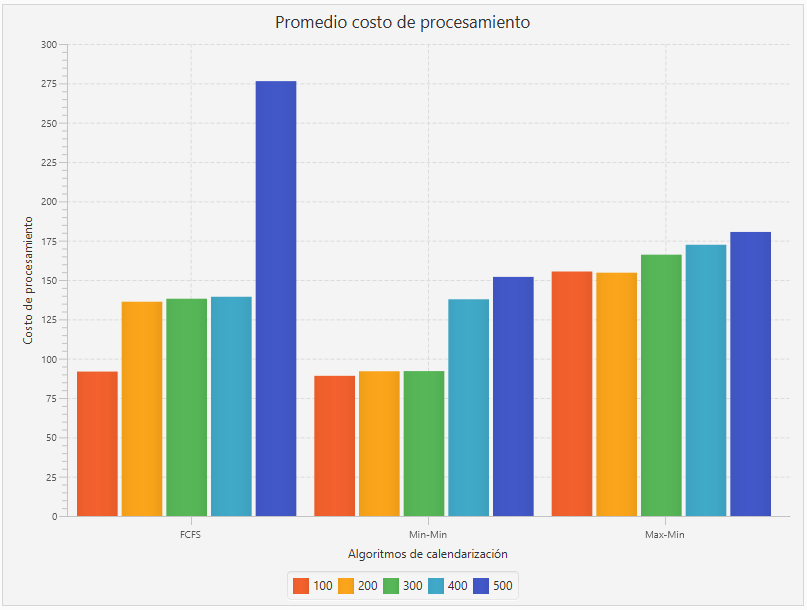
\includegraphics[scale=0.5]{media/costoproce}
\end{figure}

\bigskip
El costo de procesamiento de acuerdo a cada algoritmo se puede observar en la figura 3.2, en donde el algoritmo FCFS tiene un incremento dr'astico al realizar la prueba con 500 tareas. El algoritmo Max-Min se conserv'o sin muchos cambios a pasar de los cambios en la cantidad de tareas, mientras que Min-Min tiene un menor costo de procesamiento cuando las tareas son inferiores a 300.

\begin{figure}
	\caption{Tiempo ejecución 50 muestras FCFS}
	\centering
	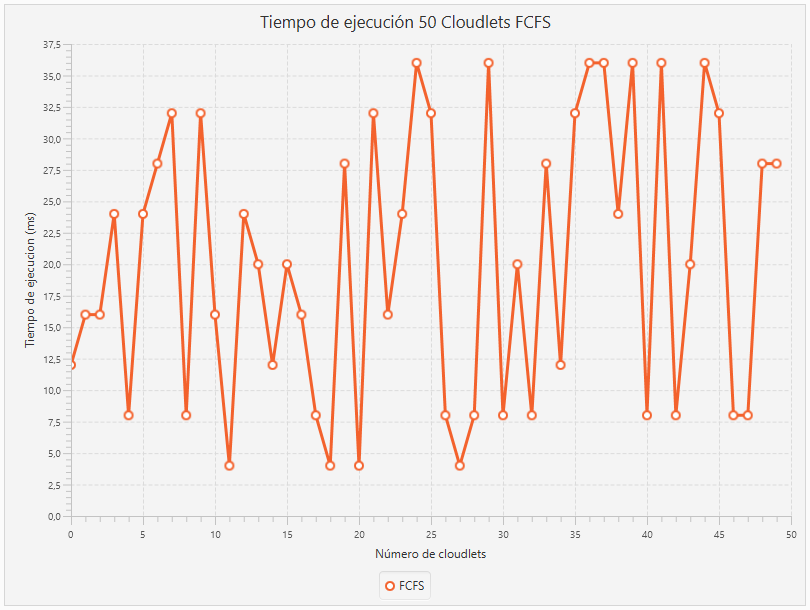
\includegraphics[scale=0.5]{media/fcfs}
\end{figure}

\bigskip
Para mostrar el comportamiento del tiempo de ejecuci'on por cada algoritmo, se tomaron 50 muestras de una simulaci'on de 500 tareas. En la figura 3.3, se puede apreciar que el algoritmo FCFS tiene un comportamiento inestable ya que algunas tareas pueden tener menor complejidad o tama'no, lo que implica una respuesta r'apida.

\begin{figure}
	\caption{Tiempo ejecución 50 muestras Max-Min}
	\centering
	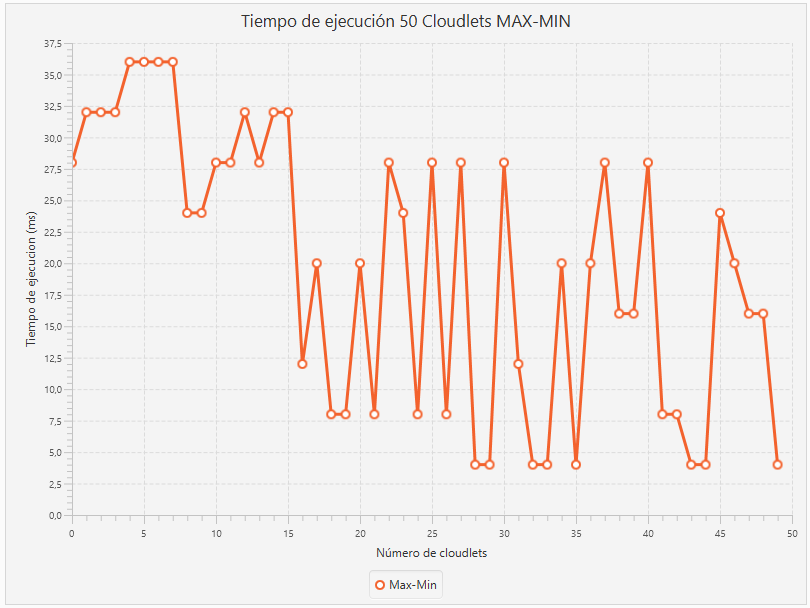
\includegraphics[scale=0.5]{media/max-min}
\end{figure}

\bigskip
 En la figura 3.4 se tiene la misma simulaci'on pero con el algoritmo Max-Min, de acuerdo a las caracter'isticas de este calendarizador, en las primeras tareas se toma un mayor tiempo en responder y va disminuyendo de manera gradual, sin embargo a'un es inestable en las 'ultimas muestras ya que no se contempla el grado de complejidad es decir el par'ametro MIPS de los cloudlets.

\begin{figure}
	\caption{Tiempo ejecución 50 muestras Max-Min}
	\centering
	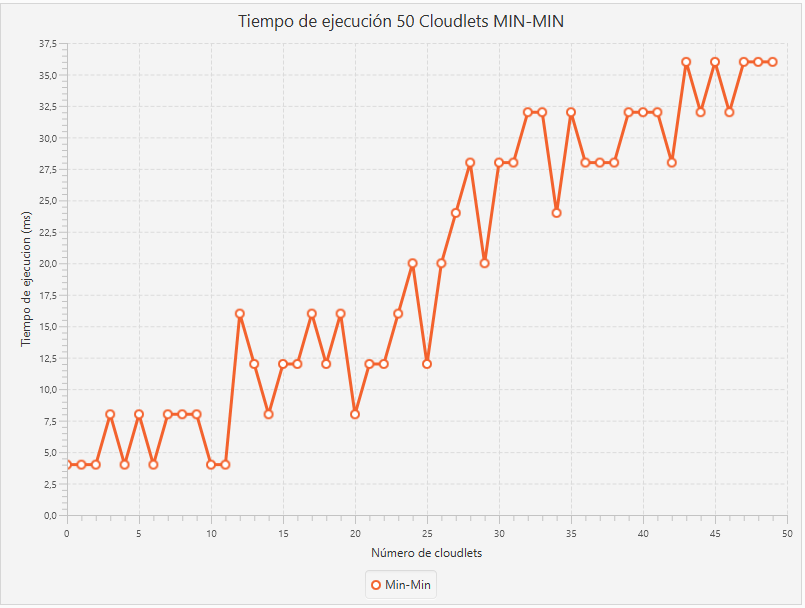
\includegraphics[scale=0.5]{media/min-min}
\end{figure}

\bigskip
Por 'ultimo tenemos el algoritmo Min-Min en el que el tiempo de ejecuci'on fue aumentando conforme se resolv'ian las tareas (figura 3.6).

\begin{table}[]
	\centering
	\caption{Desviaci'on est'andar del tiempo de ejecuci'on}
	\label{my-label}
	\begin{tabular}{@{}cc@{}}
		\toprule
		{\bf Algoritmo} & \multicolumn{1}{l}{{\bf Desviaci'on est'andar}} \\ \midrule
		FCFS & 11.00619 \\
		MAX-MIN & 8.91444 \\
		MIN-MIN & 11.25613 \\ \bottomrule
	\end{tabular}
\end{table}

Observando la desviaci'on est'andar de 'estas muestras anteriores, el algoritmo Min-Min y FCFS tuvieron m'as variaciones en las muestras con respecto a la media, mientras que el Max-Min tuvo las variaciones por debajo de las dos anteriores(Cuadro 3.5).
\chapter*{Conclusiones}
\addcontentsline{toc}{chapter}{Conclusiones}
\section*{Recomendaciones}
\addcontentsline{toc}{section}{Recomendaciones}



\bibliography{biblio}
%\renewcommand{\refname}{biblio}
\bibliographystyle{plainnat}

\chapter*{Glosario}
\addcontentsline{toc}{chapter}{Glosario}
\section*{A}
\addcontentsline{toc}{section}{A}
\begin{itemize}
	\item \textbf{Amazon:} Compa'n'ia de comercio electr'onico y servicios de computaci'on en la nube.
\end{itemize}

\section*{C}
\addcontentsline{toc}{section}{C}

\begin{itemize}
	\item \textbf{Cloud Computing:} c'omputo en la nube, tiene como objetivo ofrecer servicios a trav'es de Internet.
	\item \textbf{CloudSim:} Framework para el modelado y simulaci'on de la infraestructura y los servicios de Cloud Computing.
		
	
\end{itemize}
\section*{E}
\addcontentsline{toc}{section}{E}
\begin{itemize}
	\item \textbf{ERP:} Planificador de recursos empresariales, son sistemas inform'aticos destinados a la administraci'on de recursos de una organizaci'on.
	
	
\end{itemize}
\section*{P}
\addcontentsline{toc}{section}{P}
\begin{itemize}
	\item \textbf{Pruebas de software/hardware:} t'ecnicas cuyo objetivo es evaluar la calidad del software/hardware.

\end{itemize}




 
\chapter*{Anexos}
\addcontentsline{toc}{chapter}{Anexos}
\section*{}
\addcontentsline{toc}{section}{}

 

%%% Los cap'itulos inician con \chapter{T'itulo}, estos aparecen numerados y
%% se incluyen en el 'indice general.
%%
%% Recuerda que aqu'i ya puedes escribir acentos como: 'a, 'e, 'i, etc.
%% La letra n con tilde es: 'n.

\chapter*{Propuesta y Justificaci\'on}
\addcontentsline{toc}{chapter}{Propuesta y Justificaci\'on}

Debido a la atenci'on que se tiene en la tecnolog'ia en la nube, los centros de datos han tomado un papel muy importante para los servicios empresariales.[2] Un centro de datos est'a compuesto por miles servidores virtuales ejecut'andose en una instancia de tiempo, alojando muchas tareas al mismo tiempo el centro de datos recibe miles de peticiones a esas tareas. Es aqu'i en donde la programaci'on de tareas tiene un rol demasiado importante para el c'omputo en la nube porque influye en el rendimiento del mismo.[1] 

El problema de la calendarizaci'on pertenece a los algoritmos NP-Dif'icil, lo cual tiene un amplio rango de soluciones posibles y se toma mucho m'as tiempo de encontrar una respuesta 'optima ya que no existe un m'etodo para resolver estas inc'ognitas. Sin embargo es posible estar cerca de la mejor soluci'on contemplando algunos entornos.[2]

En esta investigaci'on se propondr'a una mejora a un algoritmo de calendarizaci'on para el caso de estudio de un sistema ERP en la nube, contemplando sus posibles escenarios y peticiones heterog'eneas.De esta manera se podr'a contar con un esquema de distribuci'on de trabajos que satisfaga las necesidades de un sistema ERP,mejorando el tiempo de respuesta y aprovechando los recursos.Con beneficios a los proveedores de servicios (SaaS) de sistemas ERP.
%%% Los cap'itulos inician con \chapter{T'itulo}, estos aparecen numerados y
%% se incluyen en el 'indice general.
%%
%% Recuerda que aqu'i ya puedes escribir acentos como: 'a, 'e, 'i, etc.
%% La letra n con tilde es: 'n.

\chapter*{Objetivos}
\addcontentsline{toc}{chapter}{Objetivos}

\section*{Objetivo general}
\addcontentsline{toc}{section}{Objetivo general}


Determinar y proponer un nuevo esquema que pueda resolver de una manera eficiente el problema de la calendarizaci'on de un centro de datos y satisfacer las necesidades de un sistema ERP en la nube.


\section*{Objetivos espec'ificos}
\addcontentsline{toc}{section}{Objetivos espec'ificos}


\begin{itemize}
\item Definir una arquitectura para un centro de datos en la nube con las necesidades de un sistema ERP.
\item Realizar la simulaci'on en base a la arquitectura del centro de datos.
\item Realizar e implementar diferentes esquemas de distribuci'on de trabajos, rescatando sus caracter'isticas principales.
\item Reunir las caracter'isticas principales y proponer el nuevo esquema de distribuci'on.
\item Aplicar el nuevo esquema de distribuci'on a las necesidades de un ERP.
\item Comparar los resultados obtenidos del nuevo esquema propuesto y de los anteriores para determinar si hubo una mejora.
\end{itemize}

%%% Los cap'itulos inician con \chapter{T'itulo}, estos aparecen numerados y
%% se incluyen en el 'indice general.
%%
%% Recuerda que aqu'i ya puedes escribir acentos como: 'a, 'e, 'i, etc.
%% La letra n con tilde es: 'n.

\chapter*{Hip\'otesis}
\addcontentsline{toc}{chapter}{Hip\'otesis}


\begin{itemize}
\item La modificaci'on de un esquema de distribuci'on mejorar'a el rendimiento de un sistema ERP en la nube.
\end{itemize}


\chapter*{Metodolog\'ia}
\addcontentsline{toc}{chapter}{Metodolog\'ia}

\begin{itemize}
\item \textbf{Simular:} Se implementar'a a manera de simulaci'on un centro de datos con un entorno en la nube, las m'aquinas virtuales y el servidor inicializador que lo conforman.
\item \textbf{Implementar:} En el centro de datos se desarrollar'an los algoritmos de calendarizaci'on que se mencionan con antelaci'on.
\item \textbf{Evaluar:} Se simular'a el comportamiento de las peticiones de un sistema contemplando los distintos escenarios del ERP y consumiendo el servicio en la nube (SaaS), para conocer el rendimiento en tiempo de ejecuci'on de los algoritmos.
\item \textbf{Mejorar:} Se propondr'a una mejora a algún algoritmo de acuerdo a las necesidades y comportamiento de un sistema ERP en la nube.
\item \textbf{Comparar:} Se realizar'a una comparativa de tiempo de ejecuci'on entre la versi'on mejorada y la original para el caso de estudio de un sistema ERP.
\end{itemize}
%%%% Los cap'itulos inician con \chapter{T'itulo}, estos aparecen numerados y
%% se incluyen en el 'indice general.
%%
%% Recuerda que aqu'i ya puedes escribir acentos como: 'a, 'e, 'i, etc.
%% La letra n con tilde es: 'n.

\chapter*{Metodolog\'ia}
\addcontentsline{toc}{chapter}{Metodolog\'ia}
%\chapter*{Plan de trabajo}
\addcontentsline{toc}{chapter}{Plan de trabajo}
\centering
\hspace*{-1.8cm}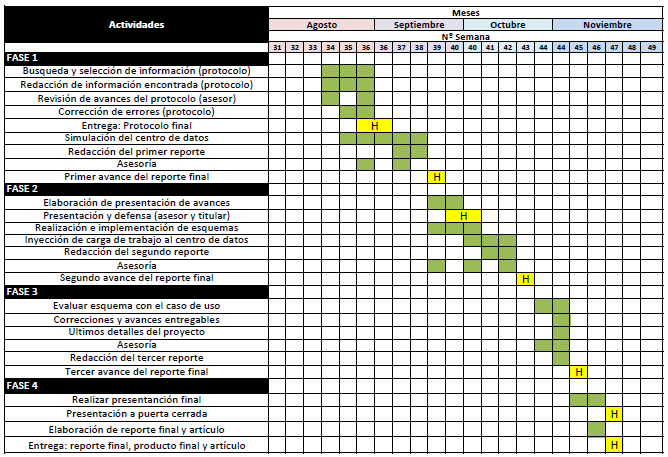
\includegraphics[]{media/trabajo}


%\include{conclu}


%% Incluir la bibliograf'ia. Mirar el archivo "biblio.bib" para m'as detales
%% y un ejemplo.



\end{document}
